\newpage

\section{Intrusion Detection System (IDS) and Intrusion Prevention System (IPS)}
IDS and IPS are services on the \opnsense\ firewall. To perform the operation, the firewall uses Suricata\footnote{\url{https://suricata-ids.org/}}. Suricata is an open-source signature-based IDS and IPS solution. Suricata is signature-based, which means that it matches the content in packets against a list or database with signatures of known strings/patterns that are suspicious.

The difference between an IDS and an IPS is that the IDS (Intrusion Detection System) is a service that is used to \textbf{detect} anomalies in the network. And the IPS (Intrusion Prevention System) is a service that is used to \textbf{block or halt} anomalies in the network.

In this section, you will learn to:
\begin{itemize}
    \item Configure an IDS.
    \item Create IDS rules.
    \item Testing if EICAR is detected.
    \item Add IPS capabilities to the IDS.
    \item Understand what the differences between IDS and IPS are.
\end{itemize}

\subsection{Enable IDS}
\warnblock{Before continuing with this task, it is recommended to add more RAM to your \opnsense\ firewall. Depending on how much memory you have on your host machine, it is recommended to increase the memory to at least 2GB. To do this, you need to shut down the firewall and edit the memory setting in VMware for the firewall client.}

It is fairly easy to enable the IDS in the firewall. Follow the following steps to activate IDS:

\setupblock{\begin{enumerate}
    \item Goto \cmd{Services --> Intrusion Detection --> Administration}.
    \item Click the checkbox besides \cmd{Enabled} to enable the IDS.
    \item Click \cmd{Apply}.
\end{enumerate}}

If everything went well, you will now see that three icons appear in the right top corner of the \cmd{Administration} page (icons like the ones in figure \ref{opnsense:ids_running}), and there will be an entry in the log that tells you that \textbf{Suricata} is running. The log can be found in \cmd{Services --> Intrusion Detection --> Log File}. Another method to check if the service is running is to go to \cmd{Lobby --> Dashboard} and check if the \textbf{Suricata} service is running.

\begin{figure}[h!]
    \centering
    
\includegraphics[width=0.15\textwidth]{Images/ids/running.PNG}
    \caption{Top right corner of \cmd{Administration} page of Intrusion Detection}
    \label{opnsense:ids_running}
\end{figure}

Now that the IDS is enabled, the next step is to configure the IDS.

\subsection{Setup IDS rule}

To create a rule, we need to download a ruleset and activate it:

\setupblock{\begin{enumerate}
    \item Goto \cmd{Services --> Intrusion Detection --> Administration --> Download}.
    \item Scroll down to the rule called \cmd{OPNsense-App-detect/test}.
    \item Mark the checkbox beside the rule and click on the \cmd{Enable selected} in the top of the menu. Now there will be an chackmark on the right side of the rule (in the \cmd{Enabled} coloumn).
    \item Click the \cmd{Download \& Update Rules}.
    \item Goto \cmd{Services --> Intrusion Detection --> Administration --> Rules} and you will see that there is one rule there (rule 7999999).
    \item Mark the rule and click on the alert box below. See figure \ref{opnsense:ids_alert}.
    \item Reload the IDS using the reload button. The middle button in the top right corner, as seen in figure \ref{opnsense:ids_running}.
\end{enumerate}}

\begin{figure}[h!]
    \centering
    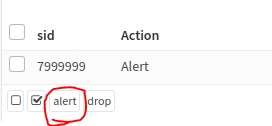
\includegraphics[width=0.3\textwidth]{Images/ids/alert_box.PNG}
    \caption{\cmd{Alert} box below IDS rules}
    \label{opnsense:ids_alert}
\end{figure}

\subsubsection*{Testing}
The \cmd{OPNsense-App-detect/test} rule is a rule that is used to test if the IDS is properly configured. It is testing against the EICAR (European Institute for Computer Anti-Virus Research) standard.

\setupblock{\begin{enumerate}
    \item Goto \cmd{Services --> Intrusion Detection --> Administration --> Alerts}.
    \item This is now empty, since we have not tested against anything.
    \item Goto \url{http://www.csm-testcenter.org/cgi-bin/eicar.txt} to test if the IDS is working.
\end{enumerate}}

\tipbox{If you get problems during testing of the EICAR rule, check if you have any other services that could prevent your firewall to access the EICAR string, such as a proxy service. Make sure the EICAR test link is using \textbf{http} and not \textbf{https}.}

\quesblock{\begin{enumerate}
    \item[44.] Try to test the IDS using a EICAR rule that has a \textbf{https} (\url{https://secure.eicar.org/eicar.com.txt})? Why do you think it is not working?
\end{enumerate}}

\subsection{Setup the IPS}
To reconfigure the IDS to an IPS there are two settings that needs to be changed:

\setupblock{\begin{enumerate}
    \item Goto \cmd{Services --> Intrusion Detection --> Administration}.
    \item Make a checkmark in the checkbox besides \cmd{IPS mode} and click on the \cmd{Apply} button.
    \item Goto \cmd{Services --> Intrusion Detection --> Administration --> Rules}.
    \item Mark the the 7999999 rule that was created earlier and hit the \cmd{drop} button (right of the alert button in figure \ref{opnsense:ids_alert}).
    \item Click the \cmd{Apply} button and reload the IDS.
\end{enumerate}}

\subsubsection*{Testing}
The \cmd{OPNsense-App-detect/test} rule is a rule that is used to test if the IDS is properly configured. It is testing against the EICAR (European Institute for Computer Anti-Virus Research) standard.

\setupblock{\begin{enumerate}
    \item Goto \cmd{Services --> Intrusion Detection --> Administration --> Alerts}.
    \item Remove all alerts using the \cmd{Delete Alert Logs} button on the right side of the date dropdown menu.
    \item Goto \url{http://www.csm-testcenter.org/cgi-bin/eicar.txt} to test if the IPS is working.
\end{enumerate}}

You should now have one entry in the log, and it should say \cmd{Blocked} in the action column.

\tipbox{If you get problems when testing this, delete cookies and reload the page you are checking and make sure that the rules are enabled.}

\quesblock{\begin{enumerate}
    \item[45.] Try to add the OPNsense social media ruleset and go to one of the well known social media sites. What happens in the log?
\end{enumerate}}

\gitblock{All of the OPNsense rules can be found in this GitHub repository:}{https://github.com/opnsense/rules}

%\subsection{Create individual rule}
% Not working atm. https://docs.opnsense.org/manual/how-tos/ips-sslfingerprint.html#

\subsection{Disabling/removing rules}
There are two different methods that can be used to remove/disabling rules for the IDS/IPS in the firewall. The first one is to disable the rules individually and the second one is to use the reverse method used when adding a ruleset to remove the ruleset.

\setupblock{\begin{itemize}
    \item Disable individually rules:
    \begin{enumerate}
        \item Goto \cmd{Services --> Intrusion Detection --> Administration --> Rules}.
        \item Remove the checkmark in the \cmd{Enabled} coloumn behind the rule(s) you want to disable.
        \item Click \cmd{Apply} and reload the service to finish.
        \item You will now see that the rule you disabled, is in a lighter grey colour.
    \end{enumerate}
    \item Disable and remove ruleset:
    \begin{enumerate}
        \item Goto \cmd{Services --> Intrusion Detection --> Administration --> Download}.
        \item Mark the ruleset you want to disable and click on the \cmd{Disable Selected} button.
        \item Click \cmd{Apply} and reload the service to finish.
    \end{enumerate}
\end{itemize}}